
\section{2a lezione di epidemiologia metodologica}

\subsection{Cronaca}


La Legionella è un microrganismo che si annida normalmente in tubature,
condutture, filtri. L'ipotesi che ci fosse la Legionella nelle torri di
raffreddamento è abbastanza plausibile. Non è però ancora chiusa
l'indagine. I casi sono diventati 38 ed i morti sono rimasti 2. I casi
ricoverati sono in via di miglioramento perchè la Legionella è sensibile
agli antibiotici. Ci devono essere un po' di accorgimenti per quanto
riguarda l'acqua, ma solo dal punto di vista delle vaporizzazioni,
perchè la Legionella ha una trasmissione aerea e non gastrointestinale.

La volta scorsa abbiamo parlato dei sistemi di sorveglianza e delle
fonti dei dati. Per quanto riguarda i dati, l'epidemiologia opera in due
direzioni:

\begin{enumerate}
\def\labelenumi{\arabic{enumi}.}
\item
  \textbf{APPROCCIO DESCRITTIVO} ai fenomeni sanitari
\item
  \textbf{APPROCCIO ANALITICO} dove l'epidemiologia è chiamata a
  identificare le cause ed i fattori di rischio
\end{enumerate}

Venendo all' esempio di Parma, il dato descrittivo è il numero di casi
di Legionellosi: 38. Questo numero però identifica il fenomeno
epidemico, ma non ci dice nulla su quelle che possono essere le cause.
Da che cosa deriva l'indagine epidemiologica analitica? Dal fatto che 35
di quei 38 casi erano concentrati in una determinata zona della città.
Questo porta ad identificare che in quell'area c'è un problema. Che
siano le torri o no, lo vedremo, ma il problema evidentemente è in
quell'area.

Nel 1874 a Londra ancora non si sapeva da cosa fosse causato il Colera e
così qualcuno diceva mangiando, altri bevendo, altri ancora respirando
quelli che venivano chiamati miasmi, cioè arie cattive maleodoranti. Ad
un certo punto, un medico di famiglia Inglese, il Dott. Snow, identificò
che la maggior parte dei casi si era verificata attorno ad una pompa
vicino a Piccadilly (non c'era ancora l'acqua corrente nelle case e si
andava ad attingere alle pompe in strada). Capì che i casi di Colera
derivavano dall'assunzione dell'acqua attinta da quella pompa. Si
identificò l'epidemia di colera 5 anni prima che fosse identificato a
Parigi, da Pasteur, il vibrione del Colera, che è l'agente eziologico.
Questo per dire che l'epidemiologia a volte identifica il problema anche
in assenza della conoscenza del meccanismo biologico. Nel caso della
Legionella si sa tutto e bisogna solo accertarsi che il patogeno sia in
quel determinato punto.

Quindi l'approccio \emph{descrittivo} sono le fotografie delle
situazioni: CHI, COSA ,QUANDO ,DOVE. Uno dei modi con cui affrontiamo
questo approccio può essere così definito: stima di nuovi casi di
tubercolosi per 100.000 all'anno, nelle diverse parti del mondo. Bisogna
ricordarsi che quando si scrive un lavoro scientifico, un rapporto, si
devono privilegiare le tabelle; quando si va ai congressi, si
privilegiano le diapositive. Come si può descrivere questa tabella?


\begin{figure}[!ht]
\centering
	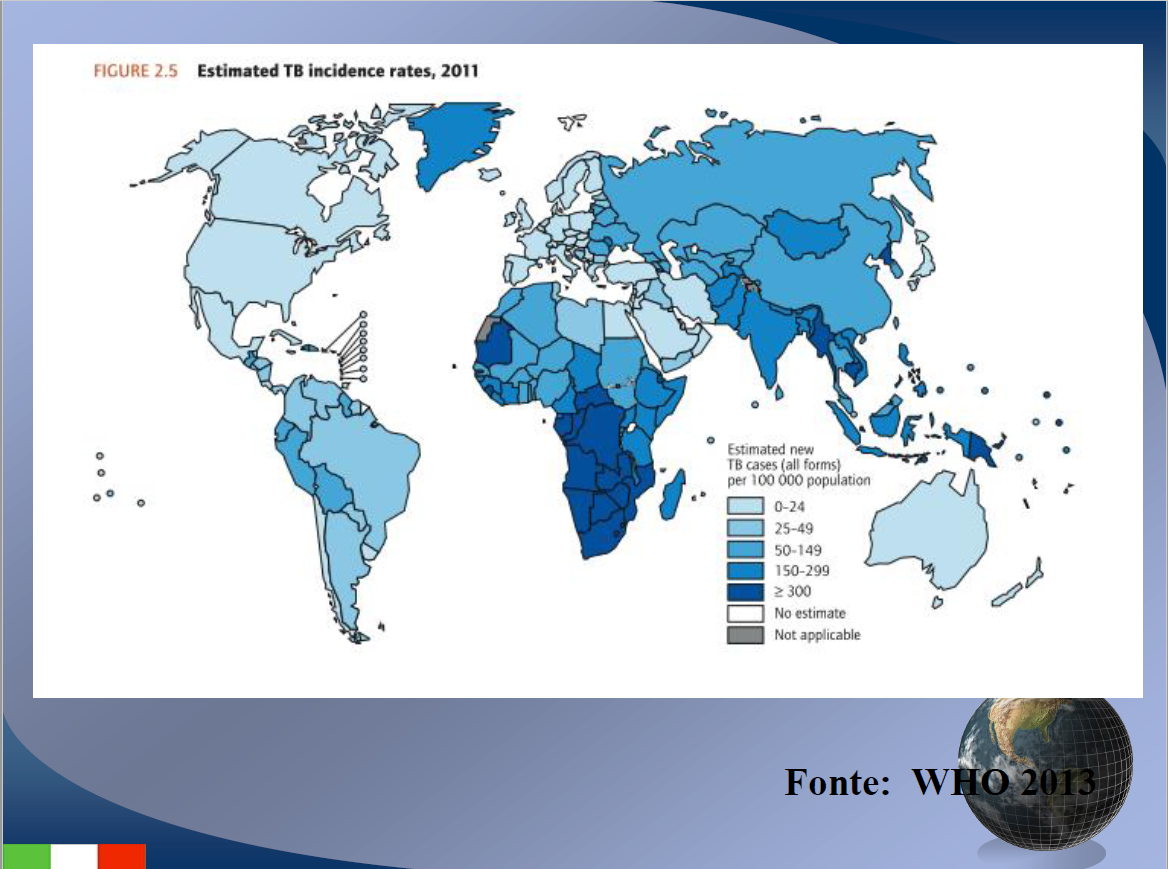
\includegraphics[width=0.7\textwidth]{03/image1.png}
\end{figure}

I paesi con più di 300 casi per 100.000 sono Africa Subsahariana,
qualche area del Sud est asiatico e la ex Unione sovietica. In realtà un
po' di TBC c'è in tutti i paesi del mondo. Non è una situazione
epidemica, ma endemica, con picchi diversi. Questo è il classico
approccio descrittivo al problema.

Se ci spostiamo alla seconda funzione dell' epidemiologia e cioè
all'approccio \emph{analitico}, andiamo a fare un'operazione leggermente
diversa , che è quella di identificare un'esposizione, che noi definiamo
così ma in realtà può essere una caratteristica individuale, una
genetica, un fattore di rischio o ambientale ecc. Generalmente noi
diciamo esposizione e misuriamo l'outcome e quindi l'effetto, cioè la
presenza e insorgenza della malattia. Di esempi ce ne sono tantissimi.

Ad es. \textbf{ESPOSIZIONE}: SINDROME METABOLICA, FATTORI EREDITARI,
ALIMENTAZIONE, SOVRAPPESO O OBESITA'-\/-\/-\/-\textgreater{}
\textbf{MALATTIA:} DIABETE.

Vedremo poi quali sono gli studi che ci permettono di fare questa
associazione, ma per il momento deve essere chiaro che l'approccio è
analitico.

Quando si va a valutare l'esposizione al fumo, si hanno dei risultati
così belli che i grafici vengono altrettanto bene a scopo didattico. In
questo caso abbiamo:

\begin{figure}[!ht]
\centering
	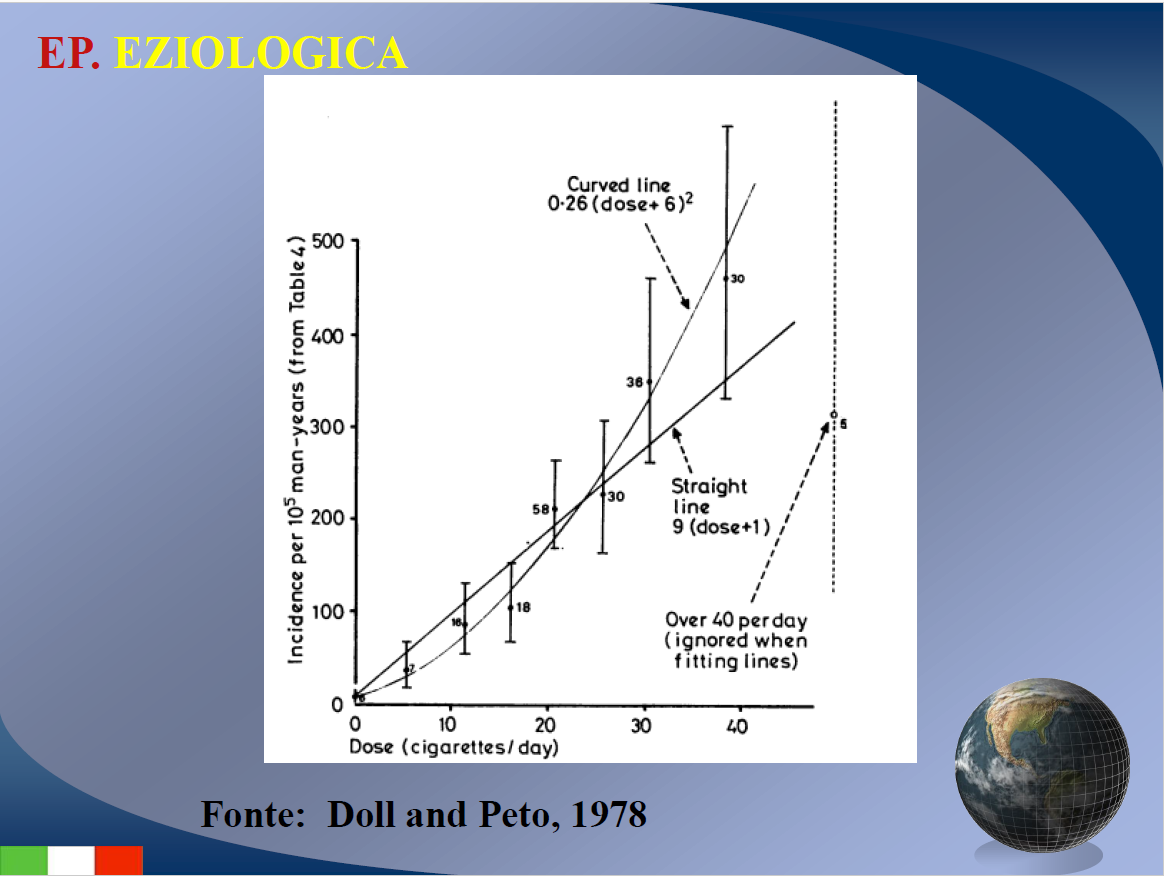
\includegraphics[width=0.7\textwidth]{03/image2.png}
\end{figure}

Sull'asse delle ascisse il numero di sigarette al giorno e in ordinata
l'incidenza, quindi la frequenza delle malattie cardiovascolari x $10^5$. I
puntini e le linee rappresentano i valori ed i limiti di confidenza. Le
rette sono le rette di correlazione. Al di là dei tecnicismi noi vediamo
che all'aumentare dell'esposizione, c'è un aumento dell' outcome e
quindi del rischio cardiovascolare.

Nei fattori di rischio c'è sempre una correlazione lineare
DOSE-RISPOSTA? Quasi sempre. Normalmente più siamo esposti, più
rischiamo, con qualche eccezione però. Ad esempio l'alcool. Se misuriamo
l'alcool e gli effetti cardiovascolari, notiamo che per piccole quantità
di alcool assunto, non solo non c'è effetto aggravante, ma addirittura,
per una ragione legata alla presenza di un maggior numero di
lipoproteine ad alta densità, l'alcool a modiche esposizioni può essere
un fattore protettivo per gli eventi cardiovascolari maggiori. Per
piccole quantità si intende mezzo bicchiere di vino a pasto. In questo
caso avremo una curva a U e non una retta lineare. Avremo che, per
piccole quantità, ci sarà un calo del rischio, via via salendo, un
rischio aumentato.

\subsection{Misure di frequenza di malattia}


\begin{figure}[!ht]
\centering
	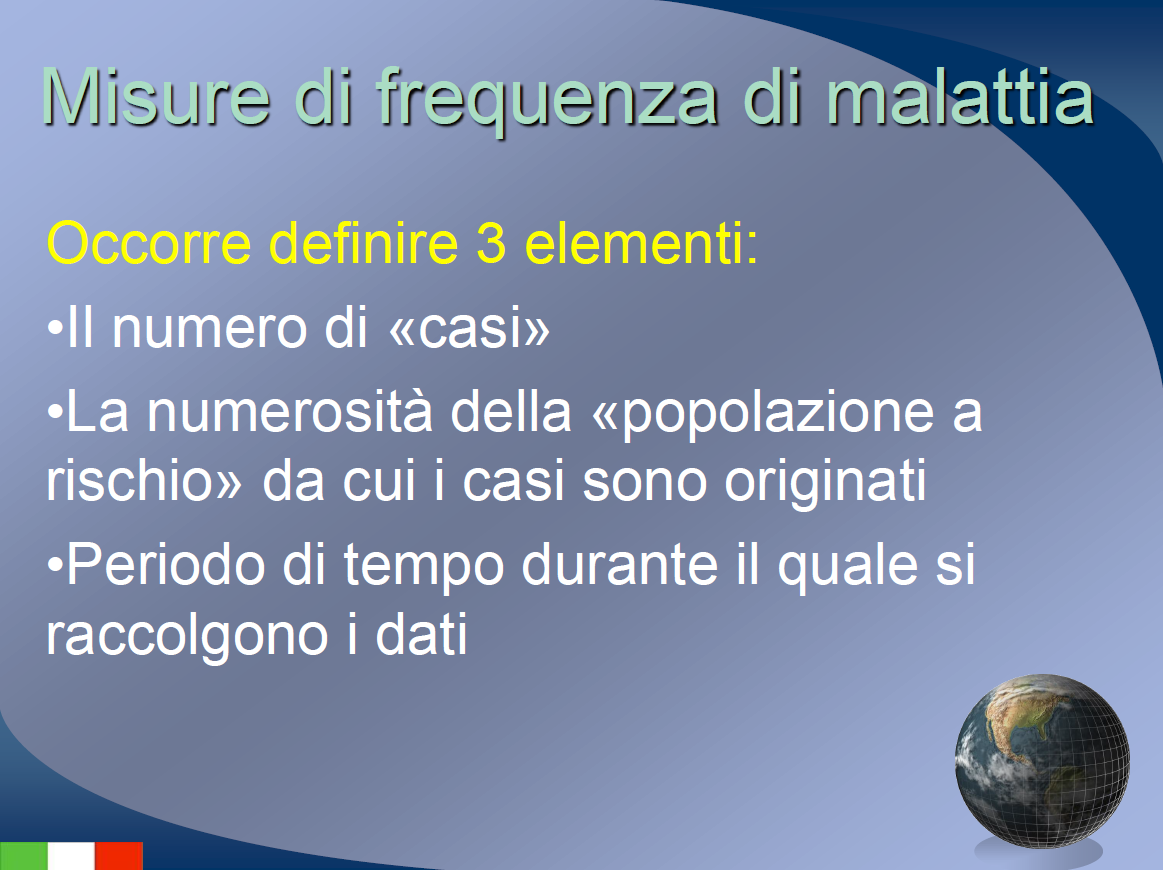
\includegraphics[width=0.7\textwidth]{03/image3.png}
\end{figure}

Vediamo ora quali sono le \textbf{misure di FREQUENZA} di un EVENTO
SANITARIO che per comodità qui chiamiamo malattia, ma potrebbe essere
morte, insorgenza di sintomi e così via.

Normalmente, misuriamo il numero di eventi in questo modo: numero di
nuovi casi per 100.000 abitanti, ma ci deve essere l'unità temporale che
nella maggior parte dei casi, per le misure epidemiologiche, è un anno .
Non è però sempre così, perchè, se misuriamo una tossinfezione
alimentare, abbiamo un periodo di incubazione talmente breve, che
potremmo calcolare l'incidenza settimanale o giornaliera. Più
frequentemente però, i dati epidemiologici, hanno l'incidenza annua.

\begin{figure}[!ht]
\centering
	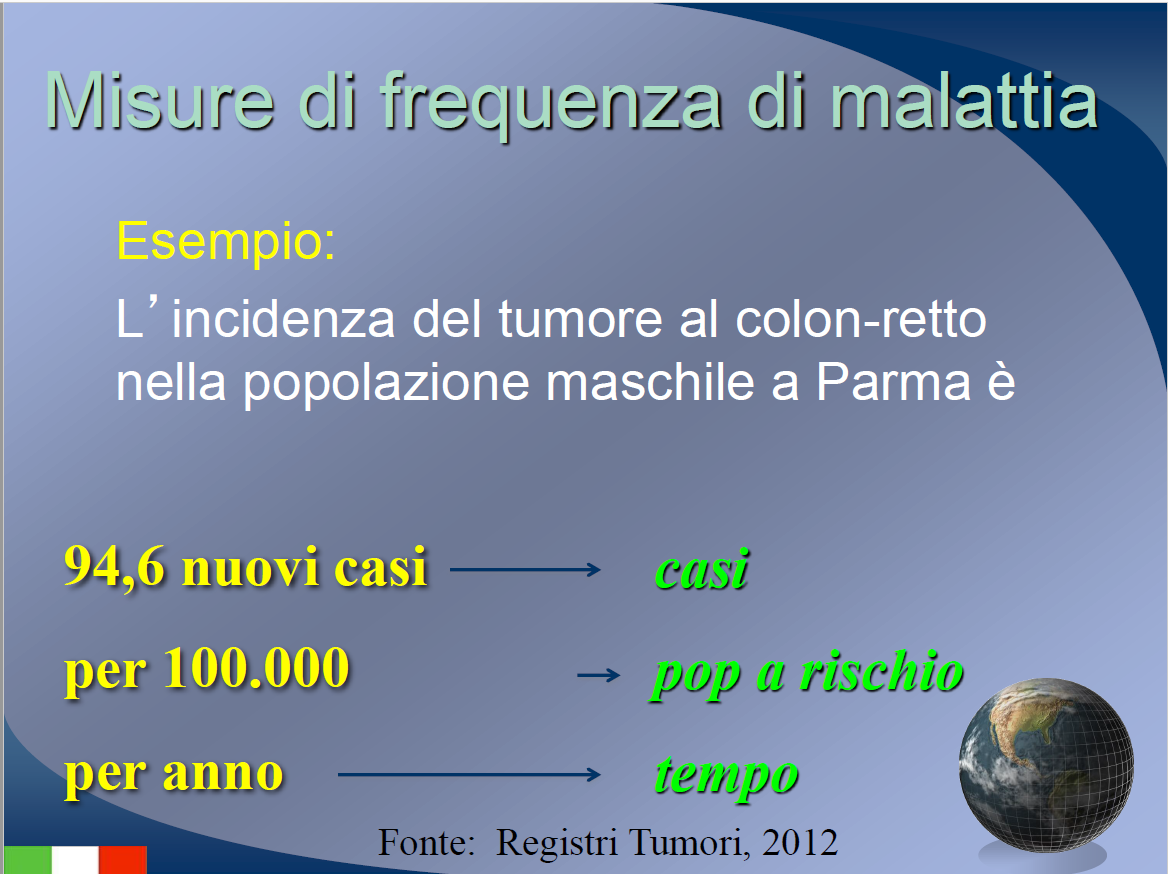
\includegraphics[width=0.7\textwidth]{03/image4.png}
\end{figure}

Questo dato, tratto dal registro dei tumori di Parma, significa che,
ogni anno, abbiamo 94,6 casi di tumore al colon-retto per 100.000.
Quindi, se la provincia di Parma ha più o meno 400.000 abitanti, ci
aspettiamo più o meno circa 379 casi di tumore al colon. Questo è un
dato descrittivo che ha una duplice funzione: da un lato valutare
l'incidenza e vedere se nel tempo sale, scende o rimane uguale;
dall'altro è utile per sapere cosa aspettarci,ovvero che la rete
ospedaliera di Parma deve essere pronta a gestire ogni anno 379 casi di
tumore al colon retto. Può sembrare una cosa non rilevante ,ma è invece
fondamentale per organizzare le chirurgie. Si spera sempre che i casi
scendano, ma potrebbero anche salire e nel caso del colon-retto i casi
sono in continua ascesa. Perchè? Una parte è legata al fatto che sta
aumentando la popolazione anziana e questo è un tumore che tende a
svilupparsi nell'età avanzata (ha il suo picco a 60 anni); un'altra è
legata all'introduzione di un elemento più raffinato per il quale oggi
contiamo più casi: lo SCREENING, la diagnosi precoce; ed infine ci sono
fattori di rischio che incidono e fanno aumentare questa patologia.

Esiste oggi un programma di screening per la ricerca di tumore al
colon-retto che si effettua tramite la ricerca di sangue occulto nelle
feci ed è richiesto dai 50 ai 70 anni con frequenza biennale. Andando a
fare centinaia o migliaia di questi test, ogni tanto trovo un tumore non
diagnosticato e ancora in fase precoce. Alla ricerca del sangue occulto,
se positivo, segue la colonscopia. Identificato il tumore, lo opero.
Ovviamente questo conta uno come caso, ma ha una prognosi decisamente
migliore rispetto a quando il paziente viene perchè ha dei sintomi. Così
però, mi aumenta l'incidenza. Quando inizio un programma di screening
devo mettere in conto che avrò un aumento dell'incidenza e che questo è
un artefatto, dovuto al fatto che anticipo la diagnosi. C'è anche
qualcuno che si chiede: se identifico un tumore di 1 cm, siamo certi che
questo maturerebbe fino a dare dei sintomi e porterebbe a morte il
paziente? Questo non si sa. Però se trovo un tumore maligno lo devo
eliminare. Anche perchè c'è un rischio di metastasi che è direttamente
proporzionale alle dimensioni della neoplasia, quindi prima la prendo,
più piccola è, migliore sarà la prognosi. Questo vale anche per la
diagnosi precoce del tumore al seno. Tutto ciò fa lievitare l'incidenza
dei tumori. Però qualcosa di positivo c'è perchè, mentre sale
l'incidenza del tumore al colon-retto, la mortalità cala.

Vediamo le \textbf{MISURE DI FREQUENZA} di una malattia.

Se misuriamo il numero assoluto di casi, questo non ci da risposte per
poter fare un'analisi comparativa con altri paesi. Abbiamo bisogno di un
denominatore. Contare i casi di per sè interessa poco, a meno che non si
tratti di una situazione come l'epidemia di legionellosi, in cui
normalmente la base è zero casi e quando inizio ad averne 10, 20, 30, mi
rendo conto dell'impatto che può avere la patologia. Normalmente si
lavora con due misure:

\begin{enumerate}
\def\labelenumi{\arabic{enumi}.}
\item
  \textbf{INCIDENZA:} \emph{numero di nuovi casi in un intervallo di
  tempo prestabilito}.
\end{enumerate}

E' una misura dinamica. Se vogliamo complicarci le cose, dobbiamo fare
un'ulteriore precisazione. Dobbiamo parlare di \textbf{INCIDENZA
CUMULATIVA e TASSO PERSONA-TEMPO.}
\begin{figure}[!ht]
\centering
	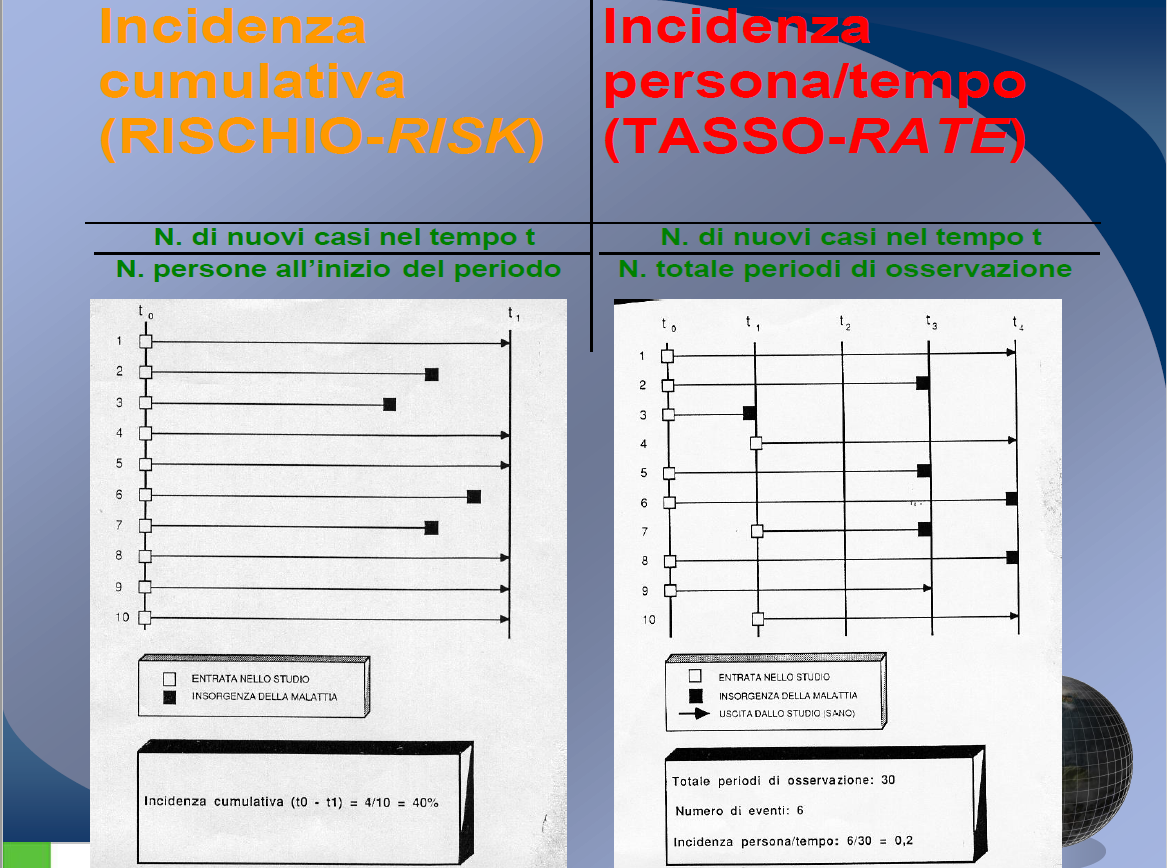
\includegraphics[width=0.7\textwidth]{03/image5.png}
\end{figure}

Il caso più semplice (incidenza cumulativa) mostra: 10 persone (il
numero è indifferente), un intervallo di tempo e un numero di casi che
insorgono in quel periodo. In questo caso 4 su 10 =\textgreater{} numero
di nuovi casi 4, persone all'inizio 10, incidenza del 40\%
nell'intervallo, che facciamo conto sia un anno. Un caso del genere si
ha quando prendiamo un numero limitato di soggetti, li seguiamo
dall'inizio di una certa età, data una certa esposizione ecc.. è un
gruppo chiuso di pazienti. Quando noi lavoriamo sulla popolazione però,
non abbiamo mai a che fare con gruppi chiusi, perchè in una popolazione
c'è gente che muore, che nasce, che migra. Non ho mai un denominatore
fisso e bloccato e allora devo fare un'operazione di approssimazione:
anzichè valutare X soggetti e il numero di casi in quei soggetti, valuto
le unità di tempo. Quindi il soggetto A ce l'ho per 4 anni
-\/-\/-\textgreater{} 0 casi per 4 anni. Nel secondo caso ho che, al
terzo anno, insorge la malattia. In realtà ho avuto la persona a rischio
per 3 anni, ma quando si ammala non è più a rischio di riammalare perchè
di solito la malattia si prende una volta sola: malattia
infettiva-\/-\/-\textgreater{} sviluppo l'immunità, malattia
cronica-\/-\/-\textgreater{} quando la prende ce l'ha per sempre. Noi
lavoriamo facendo il numero di nuovi casi diviso per il periodo di
osservazione. Quindi il dato di incidenza è quello che viene fuori nelle
statistiche perchè, quando lavoro su una popolazione, non ho mai la
coorte stabile. Tanto è vero che per calcolare il denominatore delle
popolazioni si usa il dato al 30 giugno e non al 1 gennaio o al 31
dicembre, perchè se c'è un movimento demografico, andando a prendere a
metà del periodo, ho una buona approssimazione di quante sono le persone
a rischio in quell'anno. I movimenti demografici normalmente sono lenti,
però, per essere precisi, scelgo quel periodo. Quindi alla fine avrò
incidenza persona-tempo, numero di casi, divido a periodi e lo 0,2
(della diapositiva in alto, incidenza persona-tempo) significa 20\%. Ma
rispetto a cosa? non alle persone, ma rispetto all'anno. Quindi ciascun
soggetto sano che sta un anno, ha il rischio del 20\% di sviluppare la
malattia. Il concetto non cambia, è solo un modo diverso di applicare il
tasso di incidenza. Questi dati sono di mortalità: incidenza intesa come
morte non come casi di malattia. Il tasso di mortalità non è altro che
un tasso di incidenza in cui l'evento non è l'insorgenza della malattia
ma è la morte del soggetto. Noi diciamo tasso e questo evoca un
interavallo temporale. Siamo nell'ambito dell'epidemiologia descrittiva.

\begin{figure}[!ht]
\centering
	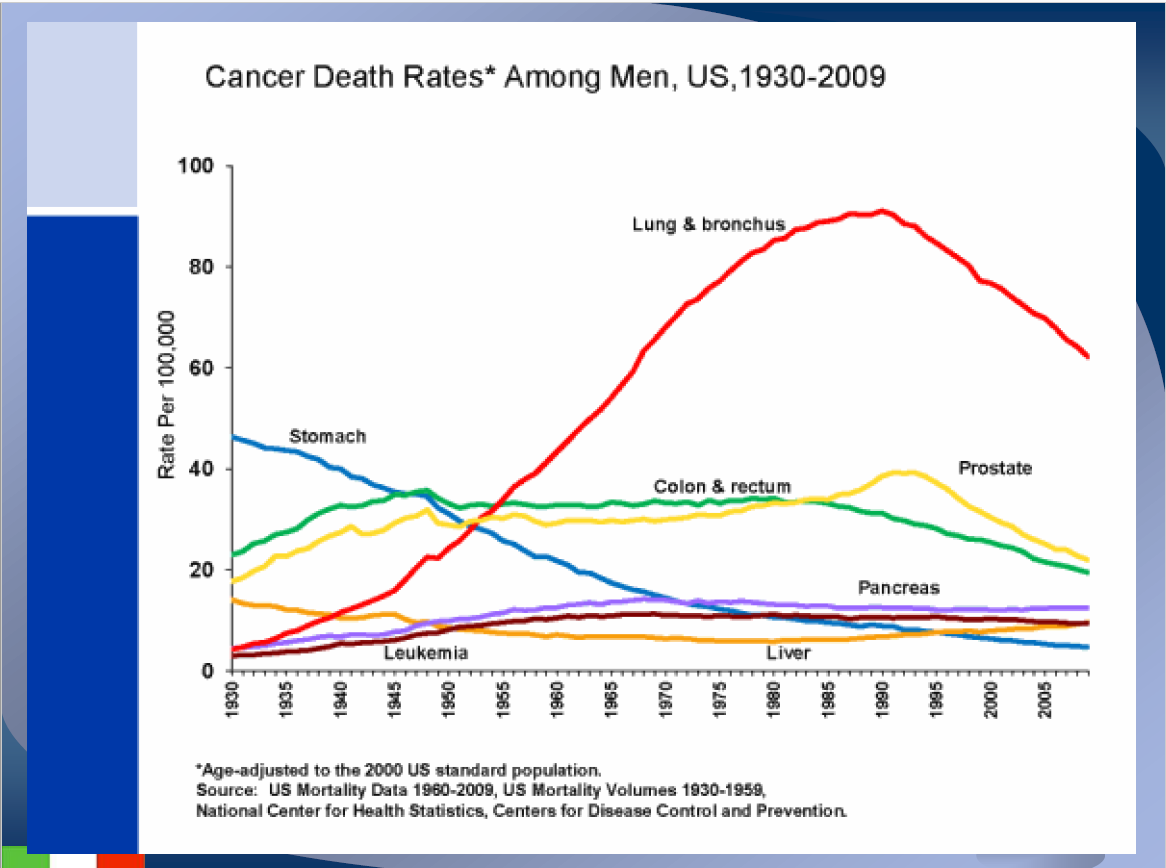
\includegraphics[width=0.7\textwidth]{03/image6.png}
\end{figure}

Questo dato, riferito agli Stati Uniti, ci dice il tasso di mortalità
per singoli tumori. Dal 1930 al 2010 vediamo un grande picco di tumori
polmonari che poi è andato calando dagli anni '90 in poi. Notiamo un
calo drastico del tumore allo stomaco dagli anni '30. I dati di
mortalità sono più attendibili e vanno indietro nel tempo molto più dei
tassi di incidenza, maggiormente difficili da calcolare, perchè mentre
sulla fonte dei dati la scheda di morte c'è sempre, sull'incidenza
potremmo non avere tutti i dati. Per il colon-retto notiamo un calo, ma
stiamo parlando di mortalità. Se avessimo i dati di incidenza, noteremmo
un aumento. Leucemia e tumore al pancreas sono in crescita. Il tumore
alla prostata ha un andamento ondulante.
\begin{figure}[!ht]
\centering
	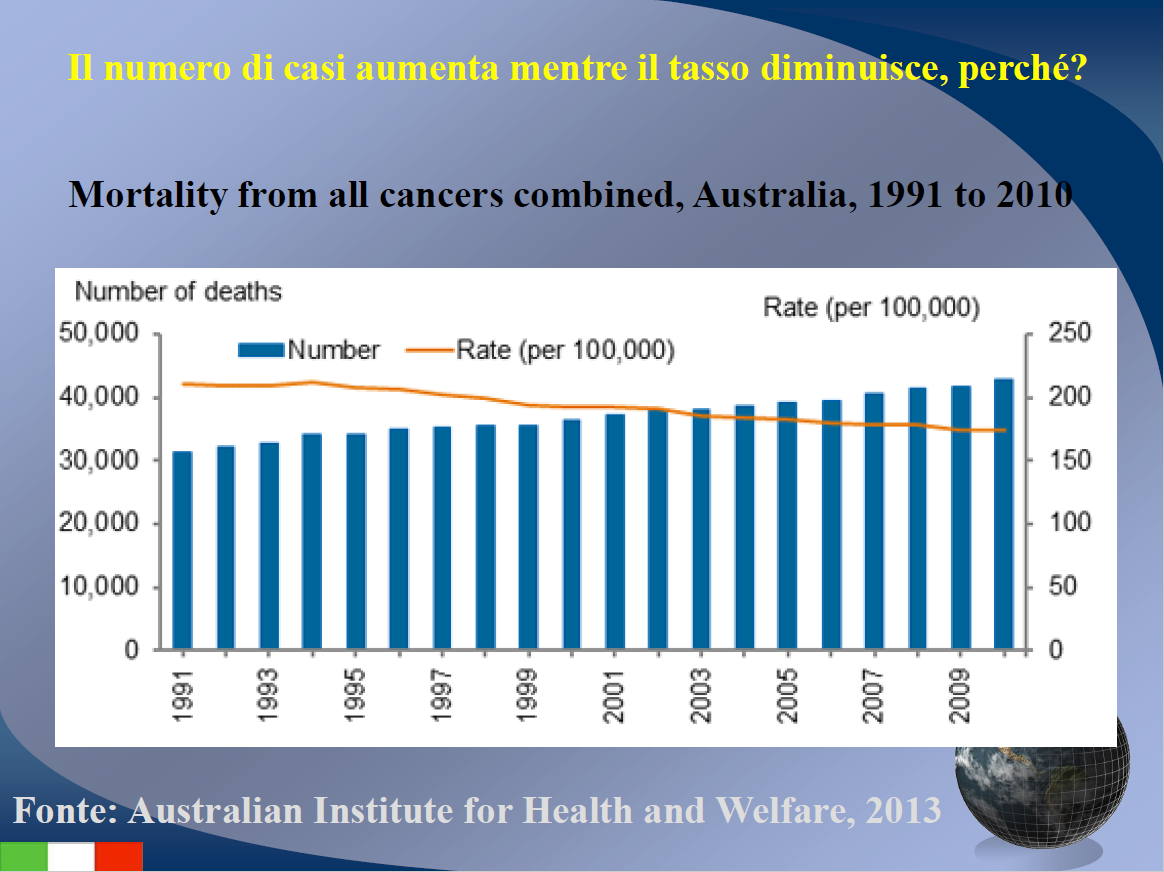
\includegraphics[width=0.7\textwidth]{03/image7.png}
\end{figure}
E' sempre bene avere presente il numero di casi, ma non bisogna
focalizzarsi solo su quelli, bensì sull'incidenza. E perchè questo?
Perchè ci fa capire che, se mettiamo insieme le mortalità per cancro
(questi sono dati australiani), possiamo avere numero assoluto in
aumento e l'incidenza in diminuzione. A noi non interessa il numero
assoluto perchè, se aumenta la popolazione, avremo più casi e non è
detto che ci sia un'incidenza maggiore. Dunque, in teoria, se la
popolazione rimanesse la stessa, il numero di casi avrebbe un trend
identico all'incidenza, ma siccome la popolazione cambia, si può vedere
la situazione in cui il numero di casi aumenta e l'incidenza diminuisce.
A quale credere? se sto facendo lo studio epidemiologico devo guardare
l'incidenza, ma se sto organizzando i servizi sanitari per curare i
malati, mi interessa il numero assoluto.

\begin{quote}
\textbf{2. PREVALENZA:} \emph{rapporto tra i casi esistenti e la
popolazione totale}.
\end{quote}

L'incidenza è un film, non è una misura istantanea, perchè devo sempre
avere un riferimento temporale. Non ci può essere un'incidenza puntuale.
Ci deve sempre essere la misura tempo che convenzionalmente per le
malattie è l'anno. Un po' come quando misurate la velocità. Misurate
km/h, m/s, c'è sempre l'intervallo temporale. La prevalenza invece è una
fotografia istantanea e fotografa la situazione esistente: numero di
casi di malattia, numero di esposti ai fattori di rischio...

Se faccio alzare la mano qui dentro a chi ha il raffreddore e mi alzano
la mano in 10, mettiamo che siete in 100 -\/-\/-\textgreater{} ho la
prevalenza del raffreddore del 10\%. Altro esempio: chi fuma? si alzano
25 mani. In questo caso ho la prevalenza del 25\%.

Classico dato di prevalenza: nell'annuario statistico 2012 si indica che
è diabetico il 5,5\% degli Italiani, valore leggermente più alto nelle
donne rispetto agli uomini; o ancora, secondo uno studio dell'OMS il
25\%-79\% degli adulti risulta in sovrappeso e il 5-30\% obeso. Sono
fotografie istantanee delle situazioni che hanno un loro significato di
rilievo istantaneo, che può essere ripetuta nel tempo. Se io fotografo
la situazione del sovrappeso in diversi anni, potrei arrivare a scoprire
differenze di un certo significato. Ad es .dagli anni '80 agli anni
2000, il sovrappeso è aumentato con tutte le conseguenze che esso può
comportare. Questo è un dato di prevalenza.
\begin{figure}[!ht]
\centering
	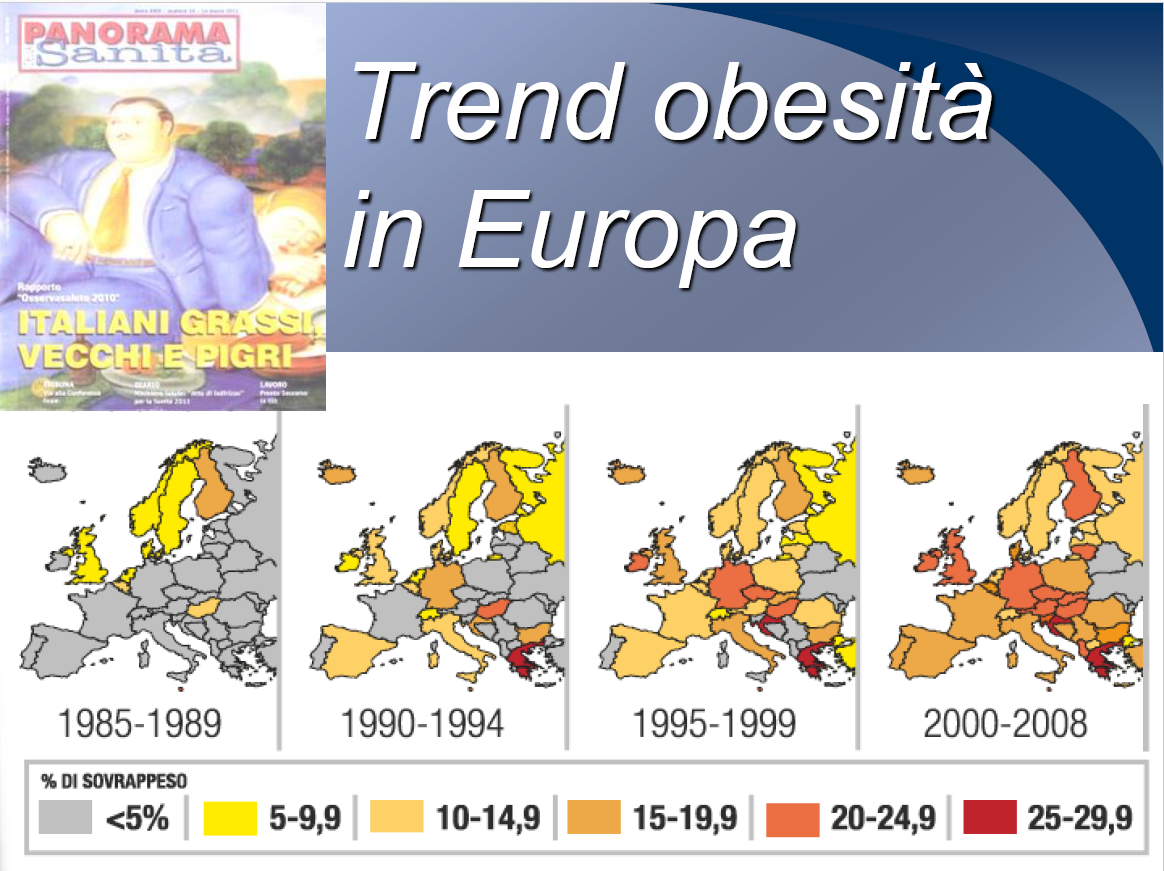
\includegraphics[width=0.7\textwidth]{03/image8.png}
\end{figure}

C'è un'immagine interessante che descrive gli Italiani come vecchi,
grassi e pigri. Se ci chiediamo quanti Italiani svolgono attività
motoria o sportiva, troviamo dei dati che imbarazzano. Meno del 50\%
degli italiani svolge attività motoria o sportiva, il che vuol dire che
abbiamo un popolo sedentario. Il problema riguarda anche i bambini e
questo è un fatto più pericoloso. Infatti il tessuto adiposo si sviluppa
in certi momenti della vita e quindi l'obesità iperplastica porta un
bambino grasso a diventare potenzialmente un adulto grasso. Un soggetto
con elevato numero di cellule adipose se le tiene come corredo della
malnutrizione dell'infanzia e della preadolescenza. Se si guardano i
bambini d'estate si nota subito come un gran numero sia in sovrappeso,
se non addirittura obeso. Si può dire che abbiano un elevato BMI
(parametro che incrocia l'altezza e il peso e determina la situazione di
normopeso, sovrappeso e obeso). C'è uno studio che dimostra che i
proprietari di cani ammalano meno di infarto o di malattie
cardiovascolari, perchè questi, bello o brutto che ci sia, devono farsi
qualche centinaio di metri al giorno per portare fuori l'animale. Queste
persone sono obbligate a farsi almeno un km al giorno. Ovviamente,
sapendo che il bilancio calorico è fatto da entrate e uscite, mangiando
di più (per un fatto culturale e sociale), l'attività motoria dovrebbe
essere adeguata. C'è dunque il problema di iperalimentazione ma anche di
attività motoria scarsa.

\begin{figure}[!ht]
\centering
	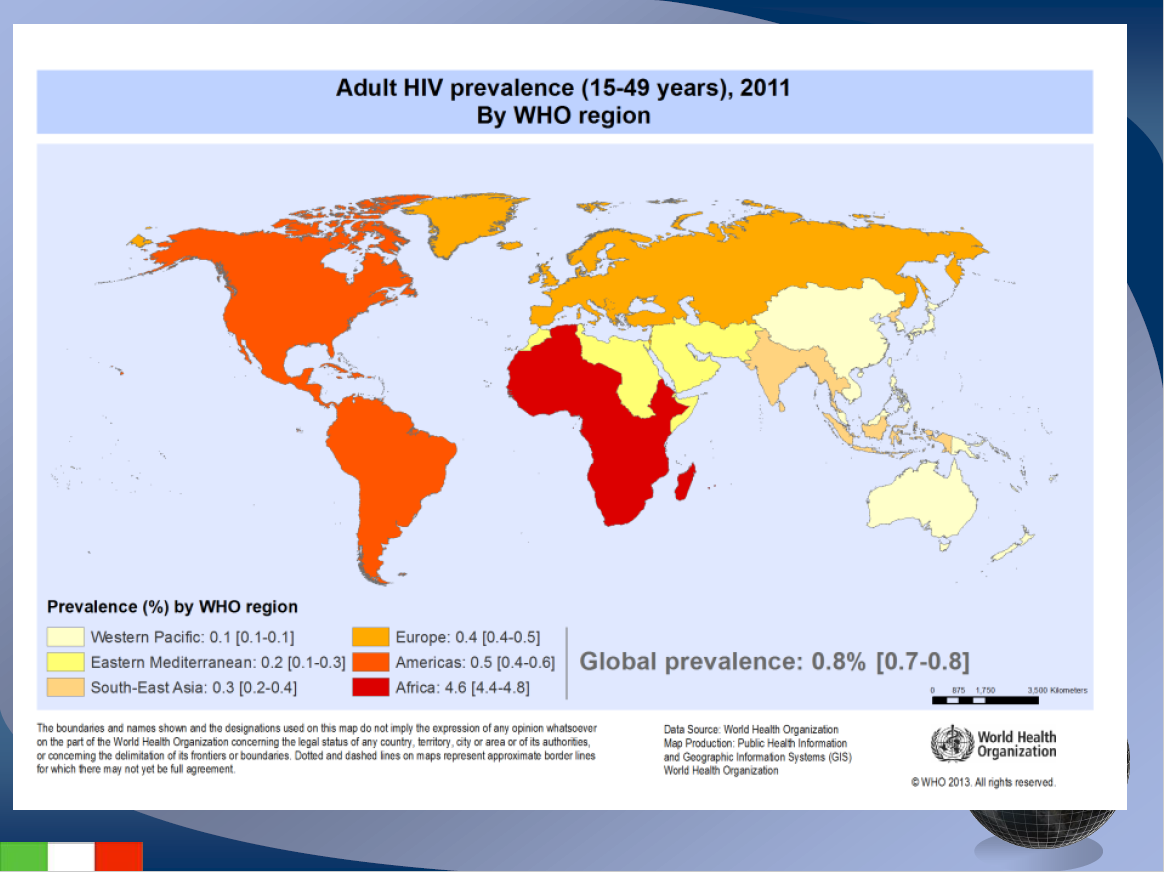
\includegraphics[width=0.7\textwidth]{03/image9.png}
\end{figure}

Prendiamo un altro esempio di prevalenza come quello dell' infezione da
HIV negli adulti, popolazione dai 15 ai 49 anni. Questa è una bella
fotografia che ci dice che oggi, la prevalenza di soggetti HIV nel mondo
è 0.8\%. Ma non è uguale dappertutto. In Europa è 0.4\%, nelle Americhe
0.5\%, in Africa 4.6\%. Alcuni paesi come Australia, Nuova Zelanda,
Giappone e Cina sono allo 0.1\%.

Ci sono poi i big killers che a livello mondiale fanno più morti e per
cui non esistono i vaccini: HIV, TBC e MALARIA. Un milione di morti o
poco meno la malaria e più o meno uguale le altre due patologie. Questi
sono dati di prevalenza, ma se andiamo a vedere l'incidenza, soprattutto
per categoria, scopriamo quali sono i principali fattori di rischio e le
principali categorie, in modo da contenere le patologie. Ad es. in
Africa i modi con cui si trasmette HIV sono 2 ancora: rapporti sessuali
non protetti e trasfusioni di sangue non controllato.

\begin{figure}[!ht]
\centering
	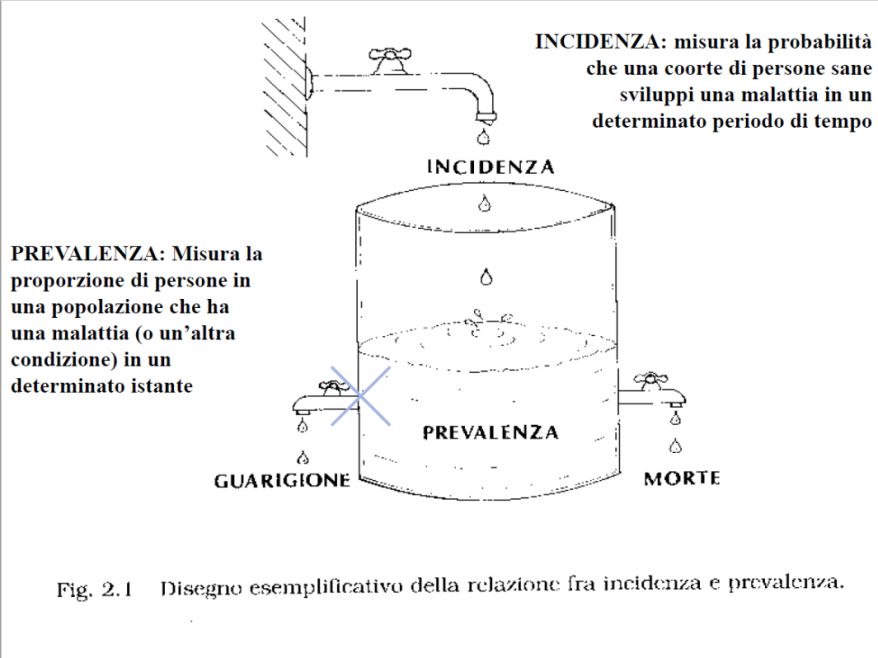
\includegraphics[width=0.7\textwidth]{03/image10.png}
\end{figure}

La botte è stata messa non per capire la differenza
incidenza-prevalenza, ma per comprendere un altro fenomeno. Quando siamo
davanti a dati epidemiologici, dobbiamo porci un problema: come si cessa
di essere un caso di malattia? o si guarisce o si muore. Per assurdo, se
ci fosse una malattia con letalità del 100\% in tempi rapidi, avrei
incidenza quello che è, ma prevalenza 0, quindi una persona appena
ammalata morirebbe (caso limite la rabbia). La rabbia non è curabile, ma
è prevenibile. Addirittura per la rabbia si può fare un vaccino post
esposizione, perchè ha un periodo di incubazione molto lungo. La rabbia
è un problema di sanità pubblica da trattare, ma oggi non dovremmo più
avere morti di rabbia. In realtà ne abbiamo pochi e solo nei paesi in
cui non si fa profilassi post esposizione. Date queste premesse, la
prevalenza della rabbia è zero, perchè come ci si ammala si muore.
Prendiamo il diabete e facciamo conto che la sua incidenza negli ultimi
30 anni non sia cambiata, anche se in realtà non è proprio così. L'acqua
che entra nella botte è sempre quella, il rubinetto della guarigione nel
diabete non c'è perchè chi lo ha se lo tiene per sempre, la letalità è
calata negli anni perchè noi, da vent'anni a questa parte, il diabetico
lo riusciamo a curare molto bene dandogli insulina. La qualità della
vita cala un po', ma il paziente riesce a sopravvivere a lungo. Cosa mi
aspetto dalla botte se riesco a stringere il rubinetto della mortalità
ed è chiuso quello della guarigione? A parità di incidenza mi aspetto
che aumenti la prevalenza. L'incidenza stabile con la prevalenza in
aumento non è negativo come dato. Questo dato ci dice che si muore meno,
quindi curo meglio il diabete. Se voglio monitorare nel tempo
l'andamento di una malattia, calcolo l'incidenza. Ma la prevalenza mi
serve per capire quanti casi sono e quindi prevedere la preparazione di
ambulatori, farmaci e personale sanitario adeguato.

\subsubsection{Misure epidemiologiche descrittive}


\begin{figure}[!ht]
\centering
	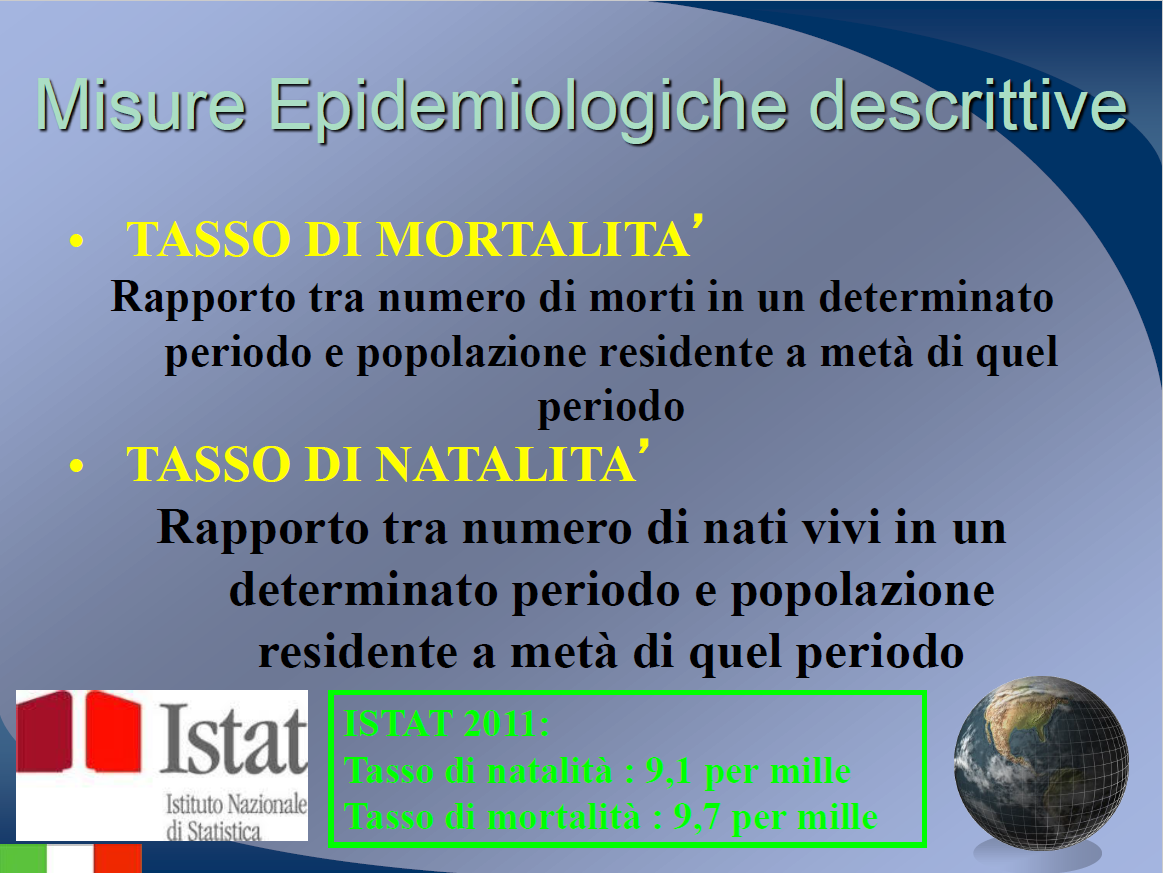
\includegraphics[width=0.7\textwidth]{03/image11.png}
\end{figure}

La mortalità è un'incidenza in cui l'evento è la morte della
popolazione. La natalità è sempre un tasso di nati vivi rispetto ai
residenti in quel periodo. Il tasso di natalità in Italia all'ultimo
censimento del 2011 è 9.1 x 1000, la mortalità 9.7 x 1000. In Italia in
questo momento muoiono più persone di quante ne nascono, però la
popolazione è sempre di 60.000.000 e questo grazie all'immigrazione.

\begin{figure}[!ht]
\centering
	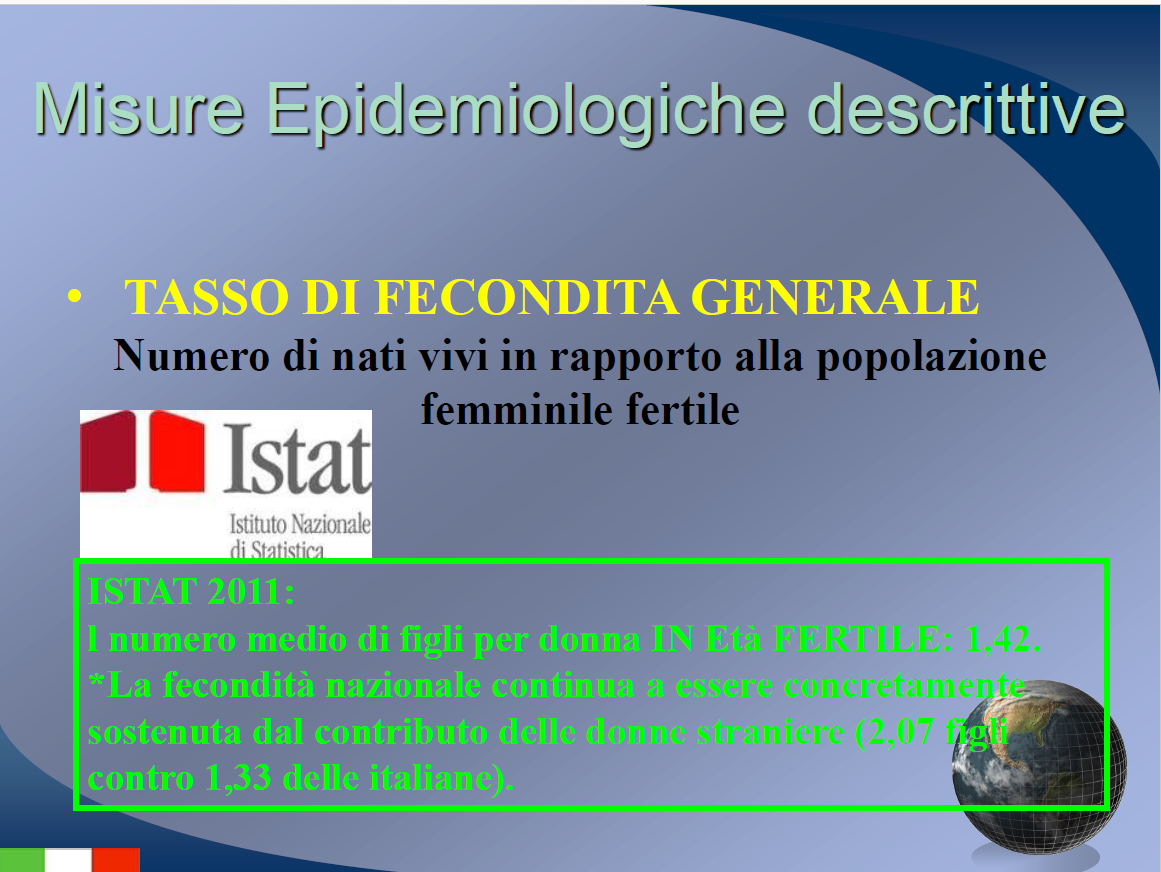
\includegraphics[width=0.7\textwidth]{03/image12.png}
\end{figure}

Se poi andiamo a misurare i tassi di fecondità (numero di nati vivi in
rapporto alle donne in età fertile), l'Italia è a percentuali dell'1.2,
con \% sotto l'1 per gli italiani e superiori per gli stranieri. La
fecondità nazionale continua ad essere concretamente sostenuta dalle
donne straniere con 2.07 figli rispetto alle Italiane con 1.33.

L'ultimo gruppo di misure descrittive sono rappresentate in questa
immagine:

\begin{figure}[!ht]
\centering
	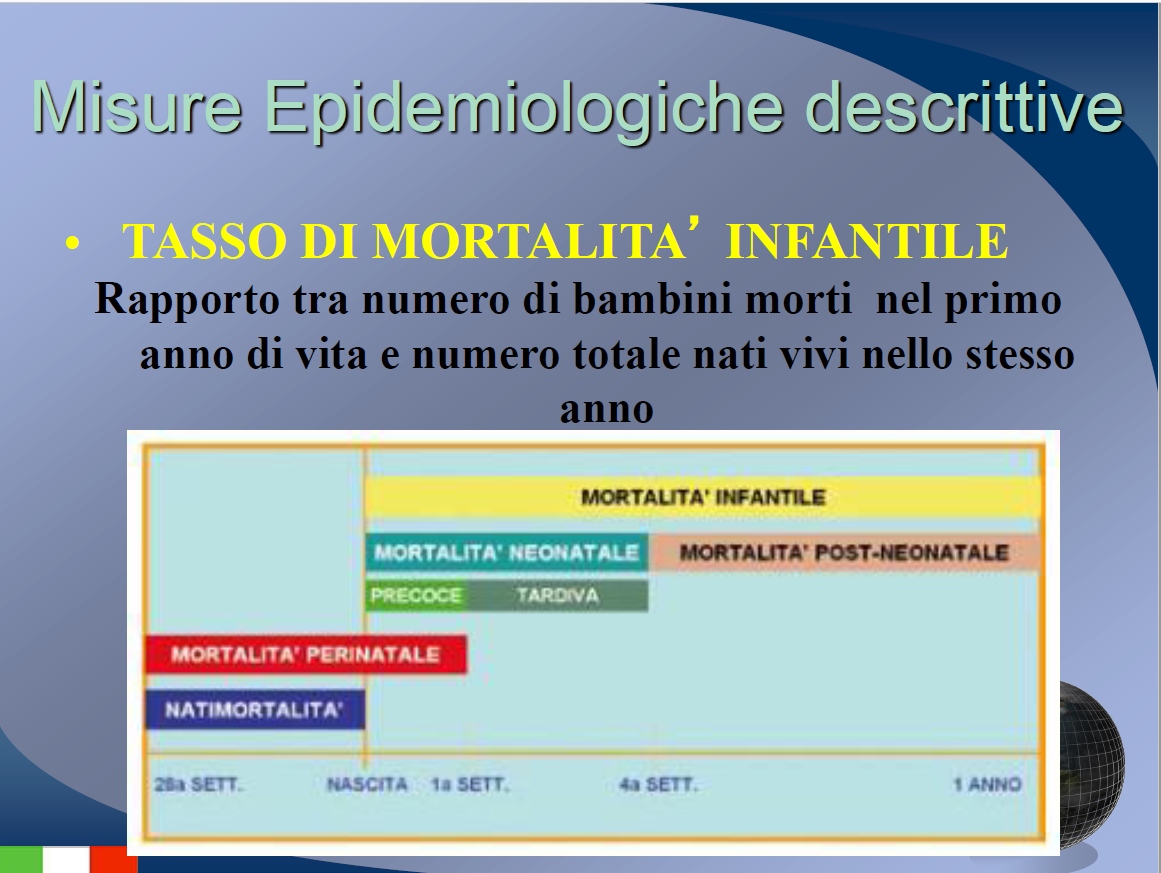
\includegraphics[width=0.7\textwidth]{03/image13.png}
\end{figure}

Ci sono alcune situazioni in cui il dato epidemiologico mi serve per
indagare alcuni fenomeni. Se prendo la \textbf{mortalità perinatale},
questa prende in considerazione le morti fetali più le morti nella prima
settimana di vita. La \textbf{nati-mortalità} tutte le morti fetali. La
\textbf{mortalità infantile}, i morti nel primo anno di vita, che a sua
volta può essere scorporata in \textbf{mortalità neonatale} nel 1\^{}
mese e \textbf{post neonatale} dal 2\^{} al 12\^{} mese. La stessa
mortalità neonatale si divide in \textbf{PRECOCE} nella 1\^{} settimana
e \textbf{TARDIVA} dalla 2\^{} alla 4\^{} settimana di vita. Tutti
questi tassi sono importanti per capire la mortalità e in più essendo
specifici per alcune categorie ci dicono diverse cose. La mortalità
infantile ad esempio è un indicatore molto preciso della situazione
igienico-sanitaria dell'area per cui noi calcoliamo il tasso. In Italia
è il 5 X 1000, in Africa il 40 X 1000. La mortalità perinatale che
analizza l'ultimo periodo di gravidanza e la prima settimana di vita, è
un indicatore dell'assistenza al parto ed alla gravidanza. Se trovo una
mortalità perinatale alta, significa che c'è qualcosa che non funziona
nell'assistenza al parto stesso. In questo caso muoiono per
malformazioni fetali, nella mortalità infantile si muore per malattie
infettive. La causa più comune di mortalità infantile in Italia è la
SIDS o comunemente detta morte in culla. Abbiamo talmente ridotto tutte
le cause di morte per altre ragioni, che è rimasto un 1,5 x 1000 su 5
legato a questa SIDS di cui in realtà non si conosce bene l'origine.
Sono arresti cardiaci improvvisi ed inaspettati.

\subsection{Misure di effetto}


\begin{figure}[!ht]
\centering
	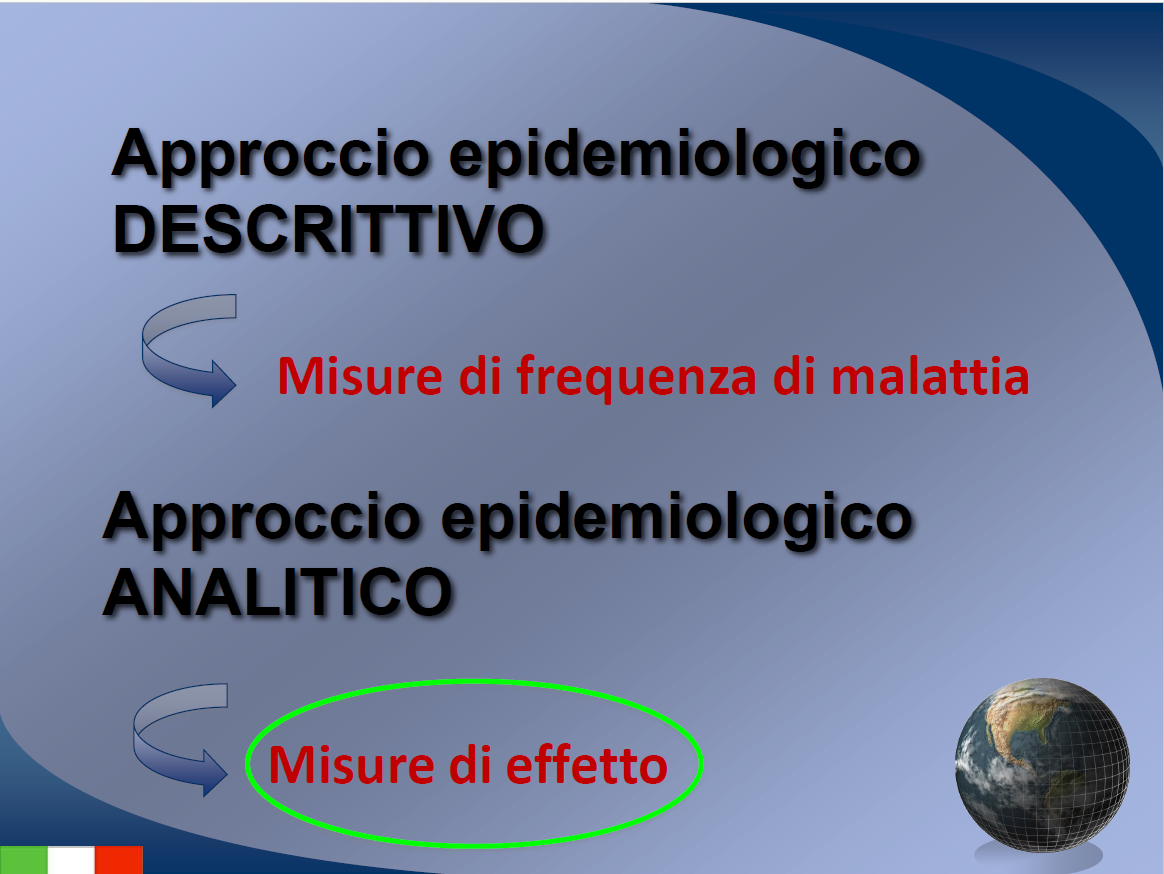
\includegraphics[width=0.7\textwidth]{03/image14.png}
\end{figure}

Veniamo ora alle \textbf{MISURE DI EFFETTO}: \emph{misurano il ruolo che
possono avere le esposizioni}.

Genericamente, sono confronti tra frequenze di malattie in gruppi
diversi. Abbiamo visto prima che ci sono le esposizioni. Se vogliamo
valutare il ruolo di un esposizione e se questa è collegata o no ad una
malattia, dobbiamo avere un secondo gruppo per calcolare la stessa
misura, l'incidenza, in chi non è esposto. Quindi se voglio calcolare il
rischio di tumore nei fumatori rispetto ai non fumatori, calcolerò
l'incidenza nel primo e nel secondo gruppo, per poter arrivare ad una
misura che si chiama \textbf{RISCHIO RELATIVO}.

\begin{figure}[!ht]
\centering
	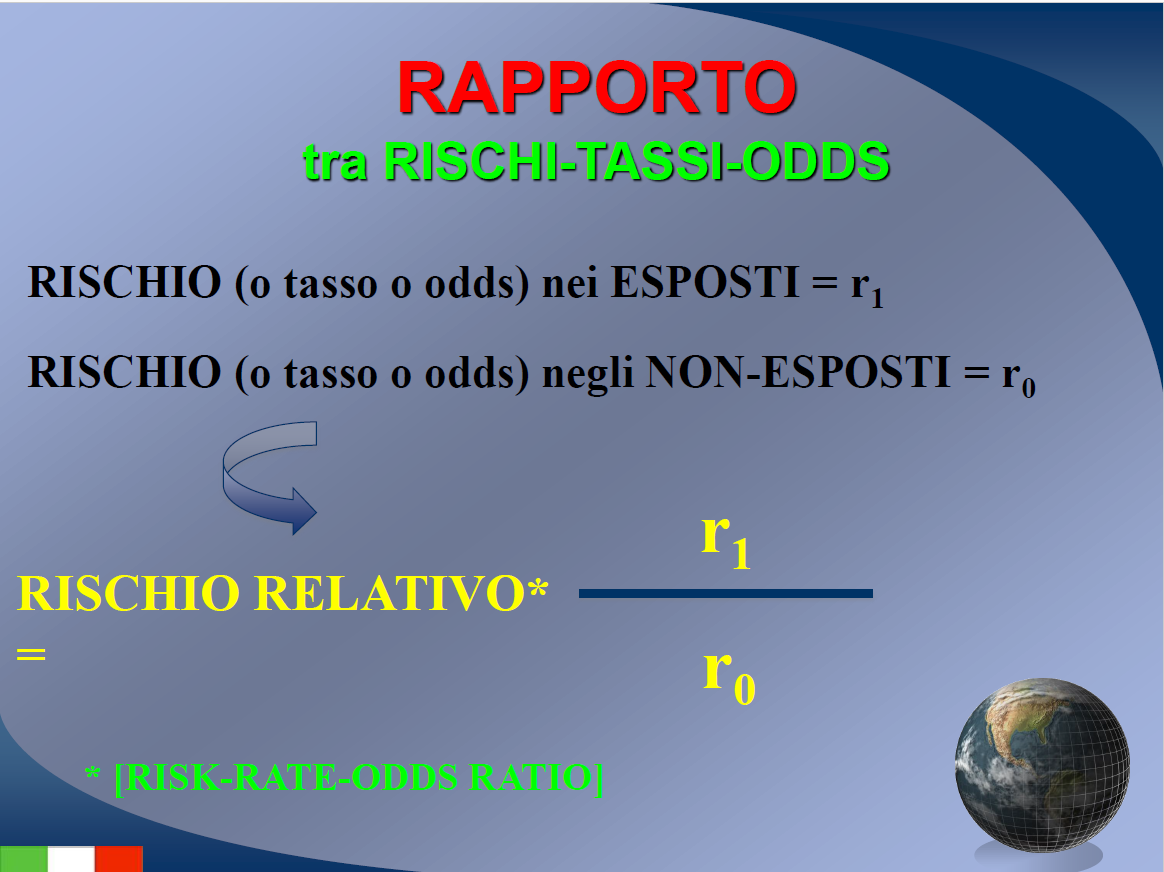
\includegraphics[width=0.7\textwidth]{03/image15.png}
\end{figure}

Il rischio relativo è l'incidenza negli esposti, diviso l'incidenza nei
non esposti. Si chiama r1/r0. Se gli esposti hanno la stessa incidenza
dei non esposti, il risultato sarà 1. Non verrà mai l'1 preciso perchè
c'è la fluttuazione statistica. Mi aspetto un numero vicino a 1 e
comunque, con le tecniche statistiche dei limiti di confidenza che
includono l'1, e che ci fanno capire come ci può essere una
fluttuazione, ma comunque stiamo intorno al'1, che significa nessun
effetto. Quando ho un rischio relativo superiore a 1, il 7 del fumo ad
esempio, cosa significa? Che i fumatori hanno un rischio di ammalare di
tumore superiore di 7 volte ai non fumatori. Ci sono anche i tumori al
polmone non associati al fumo, ma chi fuma ha un rischio maggiore, anche
in proporzione alla quantità di sigarette fumate. Il fumo da effetti a
lungo termine. il tempo di latenza per un effetto grave nel fumatore è
di 15-20 anni. Chi fuma a 20 anni non ha l'evento sanitario a 25, ce
l'ha a 45. L'epidemiologia attraverso studi sofisticati ci ha detto
un'altra cosa. L'ex fumatore non va a zero come rischio subito, ma va a
zero dopo 15 anni. Se il fumatore di adesso (23 anni) smette, a 40 anni
torna al rischio dei non fumatori. Il benefit è che il fumatore di 20
anni rischia 7 volte in più, ma 7 volte in più di una quota bassissima.
Dallo 0.1 x 100.000 diventa 0,7 x 100.000. I tumori al polmone a 20 anni
sono rarissimi e quindi c'è un maggior rischio relativo, ma un valore
insignificante in termini di rischio reale. A 40 anni le cose iniziano a
cambiare. Questo per dire che se l'abitudine viene dismessa presto,
probabilmente in termini assoluti, il rischio aggiuntivo del fumo a 20
anni è molto limitato. Molto diverso è quando il rischio si attesta a
1.1. C'è una controversia epidemiologica sulla pillola e l'aumento del
rischio del tumore al seno. Quando arriva uno studio che prova che il
rischio relativo di 1.1 è reale, in commercio c'è già una pillola con
dosaggi minori e quindi si dice che quello è il risultato della pillola
di vecchia generazione. Qualche volta abbiamo a che fare con risultati
\textless{}1. In questo caso non abbiamo a che fare con fattori di
rischio, ma l'esposizione è protettiva. Se inserisco il numero di
chilometri percorsi al giorno ed il rischio cardiovascolare, mi verrà un
risultato negativo e cioè camminare è un fattore protettivo e non un
fattore di rischio. Un esempio clamoroso: rischio relativo di 31
-\/-\/-\textgreater{} soggetti affetti da HIV hanno 31 volte più
probabilità di ammalare di polmonite di soggetti sani. E' chiaro il
perchè: HIV immunodeprime e ciò favorisce lo sviluppo di patologie
infettive. In uno studio condotto in Portogallo, il rischio di basso
peso alla nascita è 2 volte maggiore nelle famiglie a basso reddito
rispetto a quelle ad alto reddito. Il rischio relativo è 2. Poi il
fenomeno è da studiare nella sua interezza, valutando se ci sono fattori
di confondimento, perchè non è detto che il rischio relativo fornisca il
risultato (come mai pesano meno questi neonati? vengono nutriti meno?
peggio?...).

\begin{figure}[!ht]
\centering
	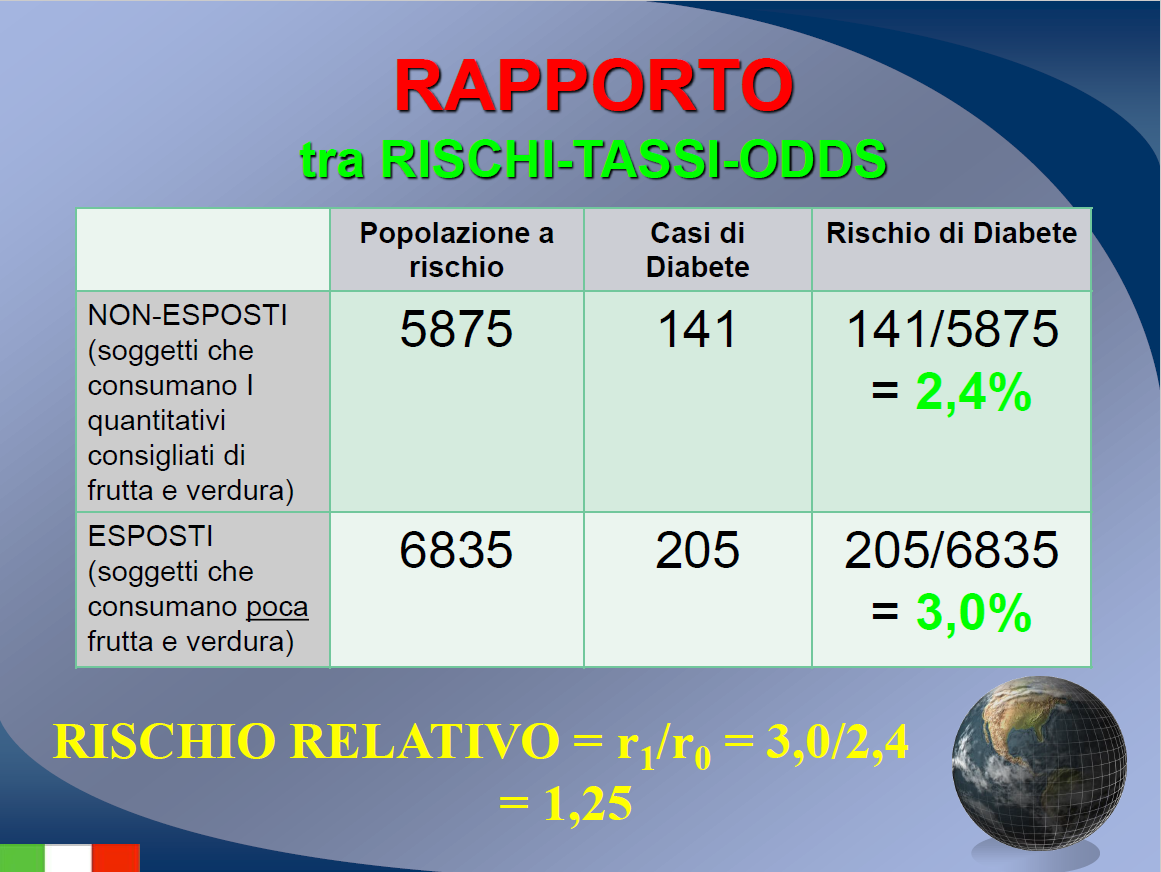
\includegraphics[width=0.7\textwidth]{03/image16.png}
\end{figure}

Guardiamo ora la popolazione a rischio per i casi di diabete. I non
esposti sono i soggetti che consumano adeguati quantitativi di frutta e
verdura, gli esposti quelli che non lo fanno. La differenza c'è, anche
se non macroscopica. Questo ci permette di individuare la frutta e la
verdura come fattori protettivi o la loro assenza come fattori di
rischio. Il rischio relativo è di 1.25. Per tutti questi rischi bisogna
poi calcolare i limiti di confidenza, questione che attiene alla
statistica. Tanto più ampio è il campione, quanto più le fluttuazioni
saranno minori. Su 10 casi le fluttuazioni saranno più ampie perchè ci
possono essere 20 casuali che influenzano i dati.

Fin qui abbiamo parlato di associazioni statistiche che indirizzano
verso una certa ipotesi, la quale è però da confermare, perchè ci
possono essere due generi di interferenze esterne: quelli che vengono
chiamati \textbf{BIAS} e \textbf{FATTORI DI CONFONDIMENTO}.
\\\\
• Il bias è una \emph{distorsione} perchè a volte sono errori di
rilevamento, a volte di conduzione dello studio, altre volte contingenti
legati al tipo di studio. Ad es. quando facciamo uno studio
caso-controllo e cerchiamo i fattori di rischio delle malformazioni
congenite nelle donne che partoriscono bambini malformati rispetto a
donne che partoriscono bambini sani e andiamo a fare l'anamnesi, la
categoria delle donne che hanno partorito un bambino malformato,
ricordano tutto quello che hanno fatto in gravidanza, mentre le altre
ricordano molto meno. Qui noi allora possiamo avere quello che in gergo
tecnico è chiamato \textbf{RECALL BIAS}. Questo non è un errore, ma è
una situazione per cui nel rilievo vedo che un gruppo di soggetti
ricorda meglio. Quando farò l'analisi dei risultati, quel gruppo
risulterà aver riferito un certo elemento che è classificato fattore di
rischio, ma che in realtà magari non lo è, perchè nell'altro gruppo c'è
una sottostima nella raccolta del dato. Questo è il motivo per cui li
chiamiamo bias e non errori.
\\\\
• Il fattore di confondimento è un altro elemento importante. Se valuto
l'andamento di un tumore nei lavoratori di un'azienda rispetto alla
popolazione generale e nell'azienda la prevalenza dei fumatori è doppia
rispetto alla popolazione generale, trovo sicuramente un rischio
relativo significativamente maggiore a uno e quello non è
necessariamente legato all'azienda, ma magari solo al fatto che lì ci
sono abitudini individuali diverse. Il ruolo del fumo in questo caso è
un fattore esterno che influenza l'interpretazione, è un fattore di
confondimento. Se quando studio i lavoratori di un azienda, calcolo
anche la prevalenza del fumo nella stessa rispetto alla popolazione
generale, il confondimento in fase di analisi dei dati lo posso
eliminare.

Dopo aver definito la presenza di bias, come facciamo a capire se
l'associazione è causale o no? Cioè se effettivamente abbiamo a che fare
con un'esposizione che aumenta la probabilità? Dobbiamo andare per
deduzione, vedere se c'è un rapporto temporale tra esposizione ed
effetto, se c'è plausibilità biologica (attenti perchè a volte i
meccanismi non li conosco), la consistenza dei diversi studi (se più
studi portano allo stesso risultato).

Riassumendo: il rischio relativo ci da la misura dell'associazione;
questa associazione per poter essere ipotizzata come causale richiede un
processo che non è statistico, ma è logico. Questo è il motivo per cui
l'epidemiologia è molto legata alla medicina. Non basta la statistica
pura.

